\chapter{Sorting of atoms}

%Tweezer arrays are especially suitable to study interactions between atoms, as distances and geometries can be changed on a run-by-run basis. However, during loading of the tweezers, sites can sometimes be filled with two atoms and subsequent light assisted collision will heat them out of the trap. This leads to an average loading of $50\%$ \cite{Cooper2018} and will make it difficult to study interactions in detail.

Tweezer arrays are especially suitable to study interactions between atoms, as arbitrary patterns can be set on a run-by-run basis. In order to load atoms into the tweezers, an ultracold atomic gas of \ce{^{39}K} is cooled in a grey molasses setup, before the tweezer beams are overlapped onto the gas \cite{Duda2017}. Each trap then has equal probability of containing either even or odd numbers of atoms. However, due to light-assisted collision \cite{Cooper2018}, pairs of bosons are heated out of the trap and lost, leaving only those traps occupied, which originally had an uneven number of atoms. This results in holes in the pattern, which makes it difficult to study interactions and requires a lot of effort in post-selection.

Consequently, it has become customary to rearrange the atoms of the system \cite{Barredo2016, Endres2016}, which is possible by using optical tweezers. Their dynamic nature allows repositioning of laser beams along arbitrary trajectories. By doing so adiabatically, atoms are moved along pre-calculated paths to fill gaps of the pattern. In the following is discussed the sorting of atoms by using \acp{aod} as the device of choice for programmatically deflecting a laser beam. Using this device, the beam can be split up, generating tweezers, and also make the beams move along paths to rearrange the atoms into the new pattern.


\section{Acousto-optically deflected tweezers}

Being able to quickly change the position of a laser beam is the most fundamental prerequisite of sorting atoms. The process has to happen on short timescales compared to the lifetime of atoms and with high accuracy. As such, it can't be accomplished using mechanical mirrors. However, light passing through a crystal can deflect off sound waves travelling transverse to the light direction through the medium. This is achieved using \acp{aod} and is discussed in the following.

\subsection{Acousto-optical effect}

The action that describes optical waves deflecting off sound waves is called the acousto-optical effect. It works similar to the Pockels effect from Section~\ref{sec:pockels_effect}, however in this case, the medium is mechanically modulated using sound. Here, planar acoustic waves travelling through a crystal modify the refractive index \cite{Saleh1991}, such that it varies with time:

\begin{align}
	n(x, t) = n - \Delta n_0 \cos{\left(\Omega t - q x\right)}.
\end{align}

Using this relation, the next step is to calculate the deflection angle off the medium. In the following, a short summary is given for the steps in \cite{Saleh1991}. The medium is broken up into slices, off which the optical wave partly reflects. Each slice has a partial reflectance amplitude $\Delta r$, depending on the refractive index $n$ and the angle of the incident optical beam with respect to the medium. The total reflectance amplitude $r$ can then be found by integrating over all slices and will carry over the dependence on the angle. By maximizing this relation, it is then found, that the angle resulting in the maximum reflectance amplitude is given by the Bragg condition:

%With this relation, it is already intuitive to see, that light entering the medium will change. 
%By assuming planar optical light passing through the medium, an approach based on calculating the reflectance in the medium using Fresnel equations \cite{Saleh1991} finds that the reflectance is maximal, whenever the incident angle $\theta_B$ of the optical wave on the sound wave meets the Bragg condition:

\begin{align}
	\sin \theta = \frac{\lambda_l}{2 \lambda_s},
\end{align}

where $\lambda_l$ and $\lambda_s$ refer to the wavelength of the light and sound waves respectively.

The maximum of the reflectance amplitude with respect to the angle is very sharp, such that in general, we can say that only if the angle between the wave vectors of the optical wave $\mathbf{k}_l$ and the sound wave $\mathbf{k}_s$ matches the Bragg condition will there be a deflected beam. Thus, another way to arrive at the Bragg condition is by finding the trigonomic relation in Figure~\ref{fig:aod_schematic}. Using

\begin{align}
	\abs{\mathbf{k}_l} &= \abs{\mathbf{k}_{l,r}} = \frac{2\pi}{\lambda_l} \\
	\abs{\mathbf{k}_s} &= \frac{2\pi}{\lambda_s},
\end{align}

it follows directly, that
\begin{align}
	\label{eq:bragg_trigonometry}
	\sin{\theta} = \frac{\abs{\mathbf{k}_s} / 2}{\abs{\mathbf{k}_{l,r}}} = \frac{\lambda_l}{2\lambda_s}.
\end{align}

\begin{figure}[t]
\centering{%
	\import{figures}{aod_schematic.pdf_tex}
	\caption{Schematic operation of an \ac{aod}.
		Light waves travelling in direction $\mathbf{k}_l$ are deflected off the sound waves with direction $\mathbf{k}_s$, resulting in a reflected beam $\mathbf{k}_{l,r}$. The deflection is successful, if the Bragg condition is met, which can be calculated via the vector relation $\mathbf{k}_{l,r} = \mathbf{k}_l + \mathbf{k}_s$.}
\label{fig:aod_schematic}
}
\end{figure}

%It is now possible to exploit this acousto-optical effect in order to deflect an optical wave by an arbitrary angle. For this, the acoustic wave is modelled as a gaussian distribution of planar waves. Then the acoustic wave has planar waves travelling in every direction, such that it is always possible to fulfill the Bragg condition, independent of the angle

%Then it will always be possible to fulfill the Bragg condition, due to the fact that there is a k-vector in every direction for the sound wave.

Using the acousto-optical effect in order to modify tweezer positions, it is necessary to break the dependence of the angle between incoming optical wave and acoustic wave, while keeping the dependence on the angle of the outgoing light. This is achieved by now modelling the sound wave as a gaussian distribution of planar waves. As such, there are waves travelling radially outwards from the origin of the sound. As a consequence of this, it will always be possible to fulfill the Bragg condition, no matter how the light enters the medium.

In Figure~\ref{fig:aod_schematic_2}, an optical beam enters a medium straight and exits on a diffracted angle $\pm \theta$, given by the Bragg condition. Using again the trigonometric relations from Equation~\ref{eq:bragg_trigonometry}, the fact that there are acoustic waves travelling in opposing directions needs to be taken into account. In the approximation where the angle is small, the Bragg condition then simplifies to:

\begin{align}
	\sin \theta_\pm = \pm \frac{\lambda_l}{\lambda_s}
\end{align}
or even simpler:
\begin{align}
	\theta_\pm \approx \pm \frac{\lambda_l}{\lambda_s}
\end{align}

\begin{figure}[t]
\centering{%
	\import{figures}{aod_schematic_2.pdf_tex}
	\caption{Schematic operation of an \ac{aod}.
		Light waves travelling in direction $\mathbf{k}_l$ are deflected off the sound waves with wave vector $\mathbf{k}_s$, resulting in a reflected beam $\mathbf{k}_{l,r}$. The deflection is successful, if the Bragg condition is met, which can be calculated via the vector relation $\mathbf{k}_{l,r} = \mathbf{k}_l + \mathbf{k}_s$.}
\label{fig:aod_schematic_2}
}
\end{figure}

\subsection{Preparation of the tweezers beams}

The deflectors used in the experiment are manufactured from Pegasus Optics and their characteristics are given in Table~\ref{tbl:pegasus_aod}.\todo{table} The \acp{aod} are provided with RF-frequencies using SMA-cables. In order to deflect in two dimensions, two deflectors are placed in series, which are turned by $\SI{90}{\degree}$ with respect to each other. This way, the first order on the first \ac{aod} will extend e.g.\ into the x-axis, while the first order of the second \ac{aod} will then extend along the y-axis. Together, exiting the deflectors will be a 2x2 grid of laser beams, which can be seen in Figure~\ref{fig:aod_pass}. These are the $(x=0, y=0)$, $(1, 0)$, $(0, 1)$ and $(1, 1)$ orders, however, only the $(1,1)$ order will be used, as this is the one that is deflected based on the sound wave placed into the \ac{aod}.

\begin{figure}[ht]
	\label{fig:aod_pass}
\centering{%
	\import{figures}{aod_pass.pdf_tex}
	\caption{Light passing through two \acp{aod} is deflected into a 2-dimensional grid. The colors refer to the optimized power going into the respective order, from lightest color being lowest power to darkest color being highest power. This way, the least amount of power goes into the (0,0) order and most into the (1,1) order.}
\label{fig:aod_schematic_2}
}
\end{figure}

The details of the configuration and characterization of the devices used in the experiment are given in \cite{Osterholz2020}.
In Figure~\ref{fig:setup_aod}, the setup used to test the programming and homogeneity of the tweezers is drawn. It consists of two laser beams that are both stabilized by measuring their power on a photodiode and using proportional-integral controllers to adjust the signal. The first laser is used for a spin-selecting atoms discussed in the next chapter and has a wavelength of $\SI{768}{\nano\meter}$. The second laser is the one used for the characterization in \cite{Osterholz2020} and sorting of the atoms, as well as testing everything regarding the tweezers in the following and has a wavelength of $\SI{795}{\nano\meter}$.

\begin{figure}[t]
\label{fig:setup_aod}
\centering
	\import{figures}{setup_aod.pdf_tex}
	\caption{Beam path to generate acousto-optically deflected tweezers. Two beams used for sorting and spin-resolved imaging are combined using a \ac{pbs}. They pass the \ac{aod} after which the beam is shaped to match the objective into the experimental chamber.}
\end{figure}

The beams then pass a $\lambda/2$ waveplate to further adjust the polarization, which in turn affects the efficiency of the \ac{aod}. The deflector, which is connected to an RF-synthesizer, then produces the 2x2 grid of laser beams. Afterwards, a $\SI{75}{\milli\meter}$ lens, projecting the center of the \ac{aod}-array, extends the beam spatially until it is collimated on the $\SI{1000}{\milli\meter}$ lens. This sets the correct beam size in order for the objective to project the beam onto the atoms.

\section{Sorting algorithms}

The ability to change the beam position at will directly leads to being able to rearrange atoms. To do so requires the knowledge about gaps in the pattern, which means when the atoms are loaded into the initial tweezers, an image is acquired, without destroying the system. From then on, atoms need to move along paths in order to fill the gaps. This has to be done adiabatically, such that no atoms are lost, but also as quickly as possible, since they have a finite, non-negligible, lifetime.

There are some sensible approximation that can be made in order to solve the optimization problem of transporting the atoms with the least amount of moves. For one, we are operating on a rectangular grid and can only move vertically or horizontally and not diagonally. Secondly, atoms that have started moving, are only released when they arrive at their destination.
The grid is separated into a target and a reservoir region. While there are still holes in the target region, the algorithm will find a way to fill the gaps using atoms from the reservoir region.

Two algorithms are presented in the following, one is based on solving a pathfinding problem and moves one atom at a time. The other uses the feature of the \ac{aod}, that allows to work on a line, trying to move as many atoms as possible at once.


\subsection{Pathfinding}

The pathfinding problem is trying to find the shortest path between two points. For sorting of atoms, this means finding the shortest set of movements to relocate an atom from the reservoir region to an empty spot in the target region.
The algorithm in question was developed by Jan Werkmann\footnote{https://github.com/PhyNerd/GridRouting} \todo{reviewers: is it ok to link the github?} and is discussed in \cite{OhldeMello2020}. One requirement for this implementation is, to reduce the number of $\SI{90}{\degree}$ turns the atom makes along the path. This results in a simplification that can be made on the algorithm, meaning that an atom moves first along one axis and then the other. This way, there are only two possible paths every atom can take. The optimal path is then the one with the least amount of obstacles in it. Here, an obstacle is simply another atom. If there is one, it segmentizes the path, moving the atom out of the way and the initial atom into its place.
\todo{explain in more detail and reference figure}

\begin{figure}[ht]
\label{fig:sorting_path}
\centering
	\import{figures}{sorting_path.pdf_tex}
	\caption{Conceptual illustration of the pathfinding algorithm for resorting. The atom tries to move into a hole but is met with an obstacle. The obstacle is first moved out of the way, after which the atom follows. The target area is then further filled with the remaining atom.}
\end{figure}

\subsection{Compression}
\label{sec:compression}

One advantage of using a digitizer as an RF-synthesizer is the ability to drive the \ac{aod} with multiple frequencies at once. This opens the door to moving multiple atoms at the same time. The compression algorithm discussed here makes use of this in order to reduce the total time of the sorting, as well as having a lower computation time with respect to the pathfinding algorithm.

The compression algorithm works by picking a full line of atoms. It then moves the selected atoms along the line towards the target area, grid point by grid point. If an atom would collide with an obstacle, that is, either another atom not currently inside an \ac{aod} tweezer, or the end of the target area, then that atom is released and not moved in the next step. This process is how in \ref{fig:sorting_compression}. When one line is finished moving according to this end condition, the next line is picked up and the process repeated. This is done first for all rows, then for all columns, and finally, all atoms are found in one corner of the grid. Doing it this way, effectively compresses all atoms in the grid into an area.

\begin{figure}[ht]
\label{fig:sorting_compression}
\centering
	\import{figures}{sorting_compression.pdf_tex}
	\caption{Sorting atoms using the compression algorithm is done by selecting a full line of atoms. They are then moved towards the left edge. An atom that meets the edge is released before the others continue moving. When the steps for the rows have are completed, the same process follows for the columns.}
\end{figure}

Due to the nature of the algorithm, there can still be holes in the target area when the sequence is finished. To overcome this problem, the pathfinding algorithm is called at the end of this step, whose runtime is favorable towards low hole numbers.

To further take advantage of the compression algorithm, a geometry is chosen, which has the target area in the center of the grid and the reservoir surrounding it, as seen in Figure \todo{fig}. As the algorithm pushes the atoms into a corner, the grid can simply be split up into four sections. Then the moves for each section is individually calculated. Ending up with moves in the row-dimension and moves in the column-dimension for each section, they can then be merged together, if they operate on the same line. As such, the sorting time of moving atoms into one corner is effectively the same as moving the atoms into the central area, by splitting it up into sections and merging the steps.

\subsection{Comparison of the two algorithms}

As the pathfinding and compression algorithm are both solving the same sorting problem, it is necessary to see a performance comparison between for the two. For this, the target area was chosen to be in the center, surrounded by the reservoir region. This gives a geometry, which has holes as close as possible to reservoir atoms, therefore giving a minimal number of movements for the pathfinding algorithm, while also making use of the performance gain that was highlighted in Section~\ref{sec:compression}.

Relevant parameters that need to be compared, are the sorting and computation time, as they need to be much slower than the lifetime of the atoms. Atom loss can also occur, whenever the atoms are transferred from the initial tweezer grid to the \ac{aod} tweezer grid used for the sorting. This way, the number of transfers are also recorded in the following.
Simulations were performed, by populating the full grid with atoms with $\SI{50}{\percent}$ probability of occupying a grid point. Then each algorithm was run over this grid and relevant parameters recorded. Simulations were run for various grid sizes, while trying to keep the fraction of number of atoms in the target area $N_{target}$ to the number of atoms in the reservoir area $N_{reservoir}$ around $\frac{N_{target}}{N_{reservoir}} \approx 0.65$. This has to be compromised for low grid sizes, as the integer nature of grid points only allows natural numbers for reservoir sizes.

The results in Figure~\ref{fig:sorting_algos} show that the compression algorithm has a faster sorting and computation time, but has to transfer more atoms into the \ac{aod} tweezer grid. However, it also shows that it scales better for increasing grid sizes. A polynomial fit is shown for the second half of the points, where the rounding issue is less present. The fit parameters are given in Table~\ref{tbl:sorting_algo_fit}, from where it can be seen, that the second order prefactor is negligible. Therefore, from the given data, the algorithms both scale effectively linear to large atom numbers.

\begin{table}[bt]
\label{tbl:sorting_algo_fit}
\centering
\begin{tabular}{l|l|l|l}
	\hline \hline
	\multicolumn{4}{c}{Pathfinding} \\ \thickhline
	& $a_0$ & $a_1$ & $a_2$ \\ \hline
	Resorting time & \num{-3.0e+02} & \num{7.2e-01} & \num{3.7e-05} \\ \hline
	Computation time & \num{-9.9e-03} & \num{1.5e-05} & \num{9.9e-09} \\ \hline
	Number of transfers & \num{-5.8e+02} & \num{1.1e+00} & \num{7.4e-05} \\ 

	\hline \hline
	\multicolumn{4}{c}{} \\
	\hline \hline
	\multicolumn{4}{c}{Compression} \\ \thickhline
	& $a_0$ & $a_1$ & $a_2$ \\ \hline
	Resorting time & \num{1.2e+01} & \num{2.8e-01} & \num{-1.1e-06} \\ \hline
	Computation time & \num{-5.0e-03} & \num{6.8e-06} & \num{8.4e-10} \\ \hline
	Number of transfers & \num{5.9e+01} & \num{5.5e-01} & \num{-2.4e-06} \\ \hline
	\hline
\end{tabular}
\caption{Fit parameters for Figure~\ref{fig:sorting_algos} by assuming parabola $f(x) = a_0 + a_1 x + a_2 x^2$, $x$ being the atom number.}
\end{table}

\begin{figure}[h]
\label{fig:sorting_algos}
\centering
	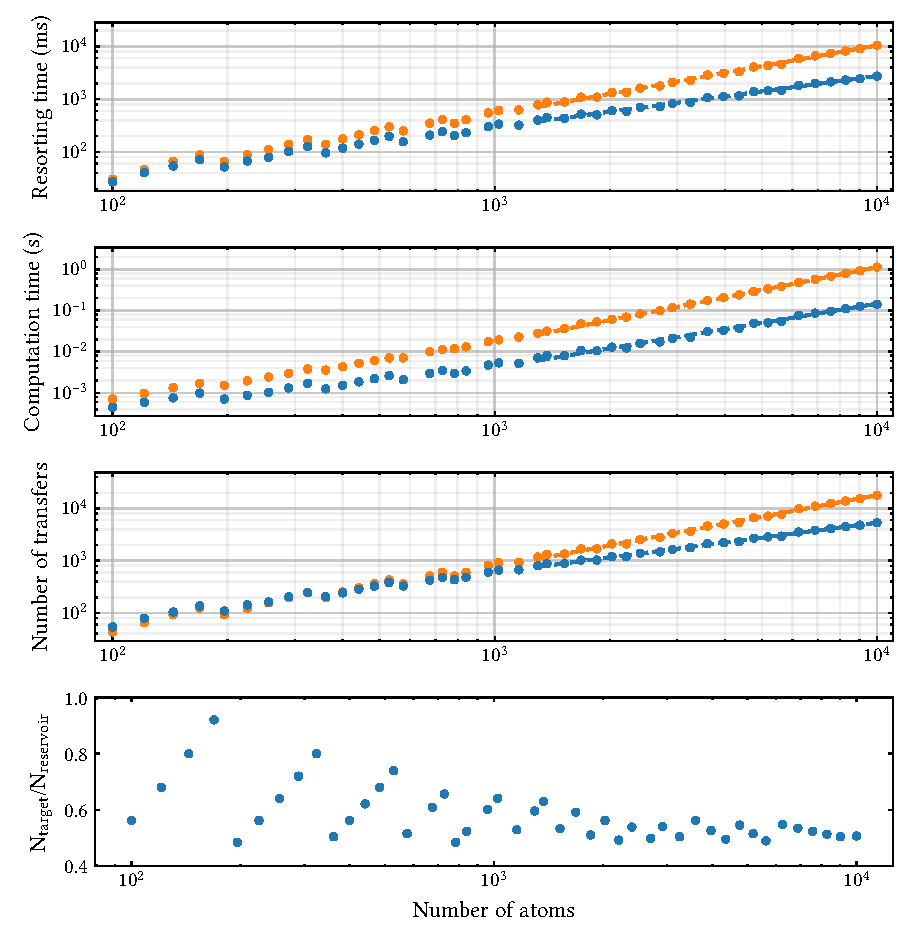
\includegraphics{figures/sorting_algos_155.pdf}
	\caption{Comparison of pathfinding algorithm (orange) and compression algorithm (blue) for sorting atoms into a target region. For each data point, 50 simulations were run and the mean of the result is shown. Standard deviation is on the size of the dots drawn and as as such are not visible. The fraction of atoms in the target versus the reservoir area are shown in the last diagram. Since only integer values are allowed for the reservoir size, the fraction between the two sees a rounding effect. For this reason, the fit is only done for the upper half of the data points, where the effect is less pronounced. The values to the fit are given in Table~\ref{tbl:sorting_algo_fit}.}
\end{figure}

\section{Driving an RF-synthesizer for arbitrary pattern generation}

One of the most powerful aspects about \acp{aod} is the fact, that a superposition of sound waves results in a superposition of light waves in the output. This way, it is possible to generate a grid of tweezers, by supplying each \ac{aod} with one or more RF-frequencies. To synthesize these frequencies, other groups have implemented solutions using \acp{pll} \todo{ref}, which can guarantee very stable frequencies. Using these, it is also possible to drive frequency ramps, however it is not possible to synthesize multiple frequencies from one \ac{pll}. Therefore using this approach it is possible to sort the atoms one-by-one, however it is not possible to generate grid patterns.

To overcome this issue, we implement a digitizer card from Spectrum Instrumentation. Doing so allows to sample arbitrary signals, for example sines, rectangles or even non-periodic ones. A \ac{dac} on the board converts the sampled points into an analog signal, which can be passed into the \ac{aod}.

\subsection{Functionality of the Spectrum driver}

The specific card used in this experiment is the Spectrum M4i.6600-x8 and its specs are summarized in Table~\ref{tbl:spec_m4i}. Communication with the card is provided through a low-level interface from the official drivers. In the following is discussed two replay modes of the spectrum card, which are standard replay mode and sequence replay mode. In single replay mode, a signal is sent onto the card, which is played back a set number of times, from start to finish. The sequence replay mode allows to upload sequences during initialization. It is then possible to play any arbitrary combination of the sequences one after another.

\begin{table}[bt]
\label{tbl:spec_m4i}
\centering
\begin{tabular}{l|l}
	\hline \hline
	Maximum sampling rate & $\SI{1.25}{\giga\hertz}$ \\
	Output level (at max sampling rate) & $\pm \SI{4}{\volt}$ \\
	Transfer speed PC to card & $\SI{2.8}{\giga\byte\per\second}$ \\
	\hline \hline
\end{tabular}
\caption{Relevant parameters of the Spectrum M4i.6600-x8 card, plugged into a PCIe x8 slot.}
\end{table}

The functionality of the card depends on two factors: The layout of the memory, and the readout speed (the sampling rate) of the memory. In the following implementation, two output channels of the spectrum card are used. Doing so, the memory is formatted, such that two bytes of channel 1 data are followed by two bytes of channel 2 data as seen in Figure~\ref{fig:spectrum_memory}. Transferring data onto the memory then requires to fill a buffer, that is, memory on the computer running the driver, that has the same layout as the spectrum card's memory.
\begin{figure}[ht]
\label{fig:spectrum_memory}
\centering
	\import{figures}{spectrum_memory.pdf_tex}
	\caption{Sampled data points are stored in a local buffer, which can then be transferred into the cards memory. The memory is effectively 1-dimensional, with two bytes for each sampled data point. Example signals are given for Channel 1 (red) and Channel 2 (blue). In the single replay mode, the data pointer will read from the first memory position until a given end point. In sequence replay mode, the data pointer will move forward, but can jump at any point based on user preference.}
\end{figure}

With this information, the structure of a program driving the digitizer card follows the following format:

\begin{minipage}{\textwidth}
In single replay mode:

\begin{itemize}
\setlength\itemsep{0.0em}
	\item Initialization phase
		\begin{itemize}
			\item Set sampling rate
			\item Set replay mode to single replay mode
			\item Allocate the buffer memory
		\end{itemize}
	\item Main loop
		\begin{itemize}
			\item Sample datapoints of the signal to play and move into the buffer
			\item Transfer datapoints from the buffer to the card
			\item Replay signal $N$ times.
		\end{itemize}
\end{itemize}
\end{minipage}

\begin{minipage}{\textwidth}
On the other hand, for the sequence replay mode, the structure is:

\begin{itemize}
	\item Initialization phase
		\begin{itemize}
			\item Set sampling rate
			\item Set replay mode to sequence replay mode
			\item Sample signals to use in the sequence programmed later
			\item Transfer signals onto the card
			\item Allocate the buffer memory (will contain information about the sequence)
		\end{itemize}
	\item Main loop
		\begin{itemize}
			\item Fill buffer with information about which singals to play
			\item Transfer buffer to the card
			\item Play sequence
		\end{itemize}
\end{itemize}
\end{minipage}

The maximum transfer speed for transferring data from the PC to the spectrum card is $\SI{2.8}{\giga\byte\per\second}$, this means that it will always be preferrable to move as few data as possible. Consequently, if possible, it is advantageous to use the sequence replay mode, as here, almost all data is already transferred in the initialization phase. All that is left to transfer, is the sequence the data pointer is following.

\subsection{Limits of using the card in the experiment}

There are some considerations to make when using a digitizer card as a driver for acousto-optical tweezers. The first one being, that the transfer of the data onto the card takes time and is given by the sampling rate. This means, that transferring data onto the card while atoms are loaded can be problematic, if the transfer time is on the order of the lifetime of the atoms, since that means that atoms are lost during this time. This can be solved by making use of the sequence replay mode, however to make use of this mode means that a large amount of memory needs to be available on the card.

In order to calculate the transfer time and memory usage, some assumptions need to be made. The assumptions and all necessary variables are summarized in Table~\ref{tbl:spectrum_assumptions}. First of all, the sampling rate is set to be maximal, at $S=\SI{1.25}{\giga\hertz}$. This follows, because the central frequency of the \ac{aod} is approximately $f_{AOD}=\SI{100}{\mega\hertz}$, therefore with the sampling rate above, one period of a sine-signal has at most $13$ sampling points. Being able to resolve the signal clearly, has the advantage to generate the frequency more accurately, therefore a good limit is $10$ sampling points per period.

\begin{table}[tb]
\label{tbl:spectrum_assumptions}
\centering
\begin{tabular}{l|l}
	\hline \hline
	Variable & Used or assumed value \\ \thickhline
	Sampling rate & $\SI{1.25}{\giga\hertz}$ \\
	Central \ac{aod} driving frequency & $\SI{100}{\mega\hertz}$ \\
	Adiabatic transfer time to new grid & $\SI{1}{\milli\second}$ \\
	Adiabatic movement time to next grid point & $\SI{1}{\milli\second}$ \\
	Grid size & 10x10 \\
	Number of tweezer transfers for sorting & 60 \\
	Number of movements for sorting & 40 \\
	\hline \hline
\end{tabular}
\caption{Variables and assumptions used in the calculations for estimation of data transfer time and memory usage under the consideration of the experiment discussed in this thesis.}
\end{table}

Assuming now, that adiabatically transferring an atom from the initial tweezer grid into the \ac{aod} tweezer grid takes $t=\SI{1}{\milli\second}$, and moving it one grid space ahead takes the same amount \todo{ref}, then the memory $M_{sig}$ one signal occupies is calculated as:

\begin{align}
	n_{points} &= S t = 1.25 * 10^6 \\
	M_{sig} &= \SI{2}{\byte} * n_{points} = \SI{2.5}{\mega\byte},
\end{align}

where $\SI{1}{\byte}$ is one byte. From the simulations of the algorithms in Figure~\ref{fig:sorting_algos}, we see that assuming a 10x10 grid, there are about 60 tweezer transfers and 40 movements for one sorting. This means 100 sequences need to be played per channel, which is $n_{seq}=200$ in total. Lastly, the memory for all signals needs to be aligned to a power of two. Therefore, from the transfer speed $v_{trf}$ in Table~\ref{tbl:spec_m4i} follows the time it takes for one transfer $t_{trf}$:

\begin{align}
	t_{trf} = \textrm{cpow2}(n_{seq} M_{sig}) v_{trf} = \SI{183}{\milli\second},
\end{align}

where the symbol $\textrm{cpow2}$ refers to rounding up to the next power of two.
These calculations set the limit for the single replay mode, however if one decides to use the sequence replay mode, the limiting factor is the memory it takes to store all possible sequences. The storage of the sequences already assumes knowledge of the composition of both channels. Therefore it is necessary to upload every relevant combination of signals for both channels. Working again with a 10x10 grid of atoms, all relevant signals are found from the following table:

\begin{table}[h!]
\label{tbl:eom_crystals}
\centering
\begin{tabular}{l|l|l}
	\hline \hline
		Signals on channel 1 & Signals on channel 2 & Usage \\ \thickhline
		10 intensity ramps up & 10 intensity ramps up & Transfer into \ac{aod} grid \\
		10 intensity ramps down & 10 intensity ramps down & Transfer out of \ac{aod} grid \\
		9 frequency ramps up & 10 constant frequencies & Move along x-axis \\
		9 frequency ramps down & 10 constant frequencies & Move along x-axis \\
		10 constant frequencies & 9 frequency ramps up & Move along y-axis \\
		10 constant frequencies & 9 frequency ramps down & Move along y-axis \\
	\hline \hline
\end{tabular}
\end{table}

Therefore there are 560 combinations and $n_{seq} = 560*2=1120$ signals to upload onto the card. Each having a size of $M_{sig} = \SI{2.5}{\mega\byte}$ results in a required memory of $M_{req}=\SI{2.8}{\giga\byte}$. More generally, on a NxM grid, the number of sequences can be calculated via
\begin{align}
	n_{seq} = 2 N M + 2 N (M-1) + 2 (N-1) M
\end{align}

and therefore the required memory is
\begin{align}
	M_{req} = \SI{5}{\mega\byte} n_{seq}.
\end{align}

With the calculations above, it is possible to apply the pathfinding sorting algorithm to the atoms in a timely manner. However for the compression algorithm, a much larger amount of signals needs to be sampled to cover all possible combinations. These will not fit on the $\SI{4}{\giga\byte}$ internal memory. Therefore, the compression algorithm can only be used when the signals are sampled during the run, when needed. To do this efficiently, parallelization on a \ac{gpu} can be used, however at the time of this writing, it has not been implemented yet.

